\documentclass[UTF8,aspectratio=169,mathserif]{beamer}
\usepackage{ctex}
\usepackage{ulem}
\usepackage{color}
\usepackage{dsfont}
\usepackage{amssymb}
\usepackage{amsmath}
\usepackage{graphicx}
\usetheme{Berlin}
\setbeamertemplate{navigation symbols}{}

\makeatletter
\newcommand{\rmnum}[1]{\romannumeral #1}
\newcommand{\Rmnum}[1]{\expandafter\@slowromancap\romannumeral #1@}
\makeatother
\newcommand{\dperp}{\perp\!\!\!\perp}

\title{$\lambda{\rm D}$中的数学}
\subtitle{Mathematics in $\lambda{\rm D}$}
\author{报告人:许博}
\date{}

\begin{document}
	\begin{frame}
		\titlepage
	\end{frame}

	\begin{frame}[shrink]{期望证明的引理}
		\begin{block}{偏序关系}
			令$\le$是集合$S$上的一个偏序关系,则$\le$满足:
			
			1. 自反性:$\forall x\in S,\ x\le x$
			
			2. 反对称性:$\forall x,y\in S,\ x\le y\Rightarrow y\le x$
			
			3. 传递性:$\forall x,y,z\in S,\ (x\le y\land y\le z)\Rightarrow x\le z$
		\end{block}
	
		\begin{exampleblock}{定义12.1.1(最小元)}
			令$S$是一个集合,以及$\le$是一个在$S$上的二元关系。对$m\in S$,如果$\forall_{n\in S}(m\le n)$,则$m$是$S$中的一个最小元。
		\end{exampleblock}
		
		\begin{exampleblock}{引理12.1.2(最小元唯一)}
			令$S$是一个由关系$\le$偏序的集合。若$S$关于$\le$有一个最小元,则这个最小元唯一。
		\end{exampleblock}
	\end{frame}

	\begin{frame}{期望的证明}
		\begin{columns}
			\begin{column}{0.44\textwidth}
				\begin{block}{非形式化证明}
					假设$m_1$和$m_2$是$S$的成员并且两者都是最小元。\\
					则$\forall_{n\in S}(m_1\le n)$且$\forall_{n\in S}(m_2\le n)$。\\
					特别地,$m_1\le m_2$且$m_2\le m_1$,由$\le$的反对称性可得,$m_1=m_2$。\\
					因此,如果$S$具有一个最小元,则这个元素唯一。
				\end{block}
			\end{column}
			\begin{column}{0.56\textwidth}
				\begin{block}{尝试在$\lambda{\rm D}$中形式化证明}
					\includegraphics[width=\linewidth]{"../imgs/12-18.png"}
				\end{block}
			\end{column}
		\end{columns}
	\end{frame}

	\begin{frame}{目录}
		\tableofcontents
	\end{frame}

	\section{相等}
		\begin{frame}[shrink]
			\begin{block}{莱布尼兹相等}
				如果两个对象在所有可能的环境中都是不可区分的,则这两个对象是相等的。
				
				形式化为:$\Pi P:S\rightarrow*_p.(Px\Leftrightarrow Py)$
			\end{block}
		
			\begin{columns}
				\begin{column}{0.5\textwidth}
					\begin{block}{相等的自反性}
						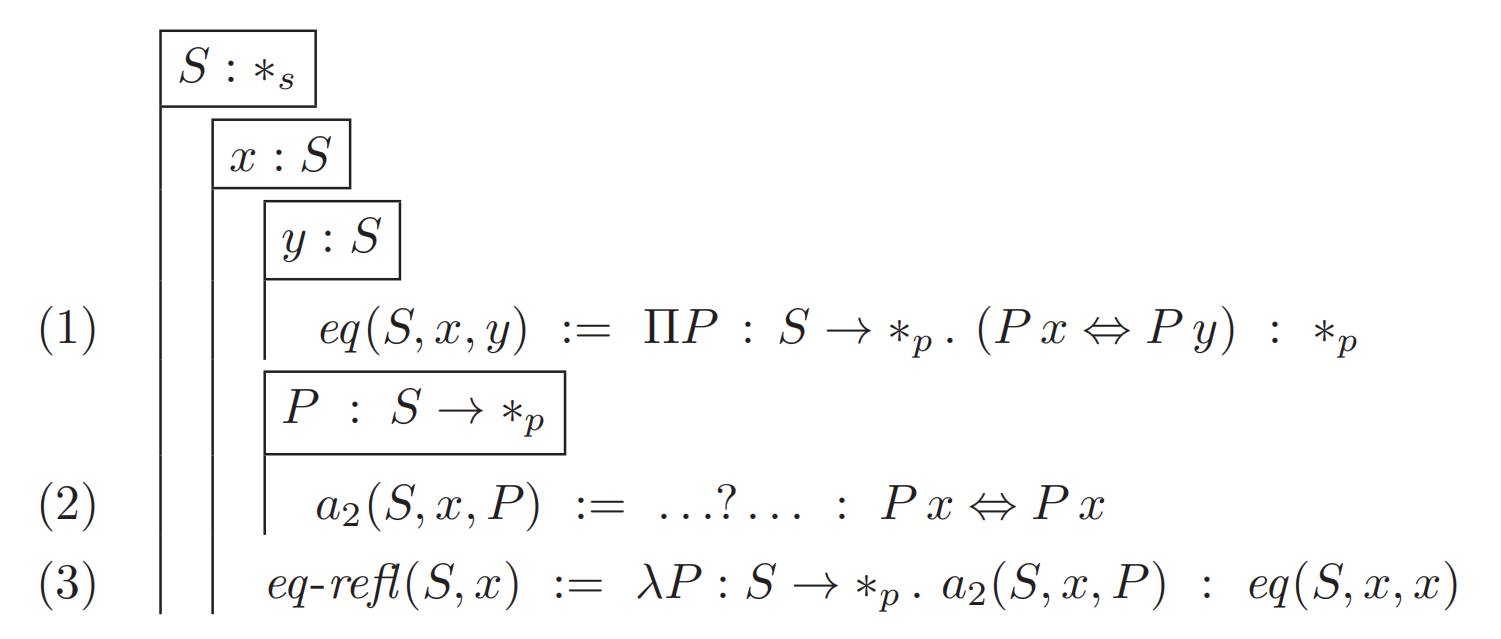
\includegraphics[width=\linewidth]{"../imgs/12-19.png"}
					\end{block}
				\end{column}
				\begin{column}{0.5\textwidth}
					\begin{block}{相等的替换性}
						对于所有在$S$上的谓词$P$,如果$x=_Sy$且$Px$成立,则$Py$也成立
						\includegraphics[width=\linewidth]{"../imgs/12-20.png"}
					\end{block}
				\end{column}
			\end{columns}
		\end{frame}
	
		\begin{frame}[shrink]
			\begin{block}{相等的一致性}
				对于所有的函数$f:S\rightarrow T$以及$x,y:S$,如果$x=_Sy$,则$fx=_Tfy$
				
				展开为:$fx=_T fy$为$\Pi Q:T\rightarrow*_p.(Q(fx)\Leftrightarrow Q(fy))$
			\end{block}
		
			\begin{columns}
				\begin{column}{0.47\textwidth}
					\begin{block}{谓词为$\lambda z:S.Q(fz)$,由替换性}
						\includegraphics[width=\linewidth]{"../imgs/12-21.png"}
					\end{block}
				\end{column}
				\begin{column}{0.53\textwidth}
					\begin{block}{谓词为$\lambda z:S.(fx=_T fz)$,由自反性及替换性}
						\includegraphics[width=\linewidth]{"../imgs/12-22.png"}
					\end{block}
				\end{column}
			\end{columns}
		\end{frame}
	
		\begin{frame}[shrink]
			\begin{columns}
				\begin{column}{0.5\textwidth}
					\begin{block}{相等的对称性}
						\includegraphics[width=\linewidth]{"../imgs/12-32.png"}
					\end{block}
				\end{column}
				\begin{column}{0.5\textwidth}
					\begin{block}{相等的传递性}
						\includegraphics[width=\linewidth]{"../imgs/12-25.png"}
					\end{block}
				\end{column}
			\end{columns}
		\end{frame}
	
	\section{序}
		\begin{frame}{形式化定义“偏序”}
			\includegraphics[width=\linewidth]{"../imgs/12-23.png"}
		\end{frame}
	
		\begin{frame}[shrink]{证明$x\le y\land y\le x\Rightarrow x=y$}	
			\includegraphics[width=\linewidth]{"../imgs/12-24.png"}
		\end{frame}

	\section{唯一存在}
		\begin{frame}[shrink]
			\begin{block}{{形式化“最小元”定义}}
				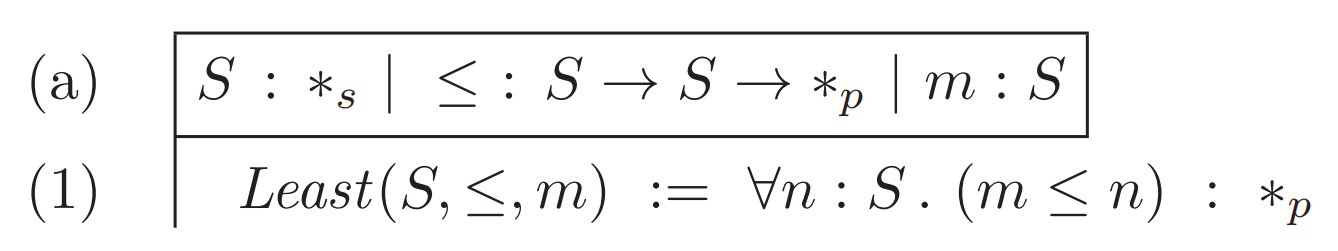
\includegraphics[width=\linewidth]{"../imgs/12-26.png"}
			\end{block}
			\begin{block}{形式化“至少存在一个”,“至多存在一个”以及“只存在一个”}
				\includegraphics[width=\linewidth]{"../imgs/12-27.png"}
			\end{block}
		\end{frame}
		
		\begin{frame}{证明仅存在一个最小元}
			$a_9:\forall m_1,m_2:S.((\forall n:S.(m_1\le_S n))\Rightarrow(\forall n:S.(m_2\le_S n)))\Rightarrow m_1=_S m_2$
			\includegraphics[width=\linewidth]{"../imgs/12-28.png"}
		\end{frame}
	
		\begin{frame}[shrink]{描述符$\iota$}
			\begin{columns}
				\begin{column}{0.5\textwidth}
					\begin{block}{\textit{a minimum}, \textit{the minimum}}
						传统数学中,通过一个名字代表一个最小元,比如说$S$关于$\le$的\textit{the minimum}。需要注意的是,如果唯一性未证明,则只能说\textit{a minimum}
					\end{block}
					
					使用描述符$\iota$命名唯一存在的元素:$\iota_{x\in S}(P(x))$表示$S$中唯一具有满足$P(x))$的成员$x$。因此,集合$S$中关于关系$\le$的\textit{the minimum}是$\iota_{s\in S}(Least(S,\le,m))$。
				\end{column}
				\begin{column}{0.5\textwidth}
					\begin{block}{定义描述符$\iota$}
						\includegraphics[width=\linewidth]{"../imgs/12-29.png"}
					\end{block}
				\end{column}
			\end{columns}
		\end{frame}
	
		\begin{frame}[shrink]{应用描述符$\iota$的一个例子}
			\begin{exampleblock}{引理12.7.1}
				令$S$是一个集合,$P$是$S$上的一个谓词,假设$\exists^1_{x\in S}(P(x))$,则$\forall_{z\in S}(P(z))\Rightarrow(z=_S\iota_{x\in S}(P(x)))$
			\end{exampleblock}
			\includegraphics[width=\linewidth]{"../imgs/12-30.png"}
		\end{frame}
	
		\begin{frame}[shrink]{使用$\iota$重新表述并证明引理12.1.2}
			\begin{columns}
				\begin{column}{0.4\textwidth}
					\begin{exampleblock}{引理12.1.2(最小元唯一)}
						令$S$是一个由关系$\le$偏序的集合。若$S$关于$\le$有一个最小元,则这个最小元唯一。
					\end{exampleblock}
					\begin{block}{重新表述}
						令$\le$是集合$S$上的偏序关系;如果$S$有最小元$x$,则$x$是$S$中关于$\le$的$the\ minimum$
					\end{block}
				\end{column}
				\begin{column}{0.6\textwidth}
					$a_{11}:\exists^1x:S.Least(S,\le,x)$\\
					$a_5:\forall z:S.(Pz\Rightarrow(z=_S\iota^u_{x:S}(Px)))$
					\begin{block}{证明}
						\includegraphics[width=\linewidth]{"../imgs/12-31.png"}
					\end{block}
				\end{column}
			\end{columns}
		\end{frame}
\end{document}